% Opcje klasy 'iithesis' opisane sa w komentarzach w pliku klasy. Za ich pomoca
% ustawia sie przede wszystkim jezyk i rodzaj (lic/inz/mgr) pracy, oraz czy na
% drugiej stronie pracy ma byc skladany wzor oswiadczenia o autorskim wykonaniu.
\documentclass[inz,longabstract]{iithesis}

\usepackage[utf8]{inputenc}

%%%%% DANE DO STRONY TYTUŁOWEJ
% Niezaleznie od jezyka pracy wybranego w opcjach klasy, tytul i streszczenie
% pracy nalezy podac zarowno w jezyku polskim, jak i angielskim.
% Pamietaj o madrym (zgodnym z logicznym rozbiorem zdania oraz estetyka) recznym
% zlamaniu wierszy w temacie pracy, zwlaszcza tego w jezyku pracy. Uzyj do tego
% polecenia \fmlinebreak.
\polishtitle    {Realistyczny rendering krajobrazów leśnych\fmlinebreak generowanych proceduralnie}
\englishtitle   {Realistic rendering of procedural generated forest landscapes}
\polishabstract {Strzeszczenie po polsku\ldots}
\englishabstract{English abstract\ldots}
% w pracach wielu autorow nazwiska mozna oddzielic poleceniem \and
\author         {Bartosz Rudzki}
% w przypadku kilku promotorow, lub koniecznosci podania ich afiliacji, linie
% w ponizszym poleceniu mozna zlamac poleceniem \fmlinebreak
\advisor        {dr Andrzej Łukaszewski}
%\date          {}                     % Data zlozenia pracy
% Dane do oswiadczenia o autorskim wykonaniu
\transcriptnum {291481}                     % Numer indeksu
\advisorgen    {dr Andrzeja Łukaszewskiego} % Nazwisko promotora w dopelniaczu
%%%%%

%%%%% WLASNE DODATKOWE PAKIETY
%
%\usepackage{graphicx,listings,amsmath,amssymb,amsthm,amsfonts,tikz}
\usepackage{graphicx, amsmath,gensymb}
%
%%%%% WŁASNE DEFINICJE I POLECENIA
\graphicspath{{./pictures/}}
%\theoremstyle{definition} \newtheorem{definition}{Definition}[chapter]
%\theoremstyle{remark} \newtheorem{remark}[definition]{Observation}
%\theoremstyle{plain} \newtheorem{theorem}[definition]{Theorem}
%\theoremstyle{plain} \newtheorem{lemma}[definition]{Lemma}
%\renewcommand \qedsymbol {\ensuremath{\square}}
% ...
%%%%%

\begin{document}

%%%%% POCZĄTEK ZASADNICZEGO TEKSTU PRACY
\chapter{Wprowadzenie}
    Pracy skupia się na zbadaniu i zastosowaniu dwóch pojęć z dziedziny grafiki komputerowej: realistyczny rendering i generowanie proceduralne. 
    
    Pierwsze zagadnienie dotyczy przedstawienia wcześniej przygotowanego modelu w sposób zrozumiały dla człowieka. Modelem może być plik opisujący kształt dzbanka. Przykładowa reprezentacja to zbiór trójkątów rozmieszczonych w przestrzeni z uwzględnieniem dodatkowych informacji takich np. kolor. Rendering takiego modelu polegałby na zamianie wszystkich tych danych na obraz, który mógłby być pokazany człowiekowi. O realistycznym renderingu możemy mówić wtedy, kiedy stworzony przez nas obraz przypomina prawdziwy dzbanek, który chcieliśmy zamodelować. 
    
    Generowanie proceduralne skupia się na tworzeniu modeli przy pomocy algorytmów. Człowiek może wpływać na finalny produkt przy pomocy zmiany parametrów jednak nie uczestniczy w samym procesie tworzenia. Jest to bardzo wydajna metoda pozwalająca na tworzenie nieskończenie wielu różnych modeli o zadanych właściwościach jak np. rośliny.
    
    Celem programu napisanego w ramach tej pracy jest generowanie prostego krajobrazu leśnego, a następnie względnie realistyczny rendering stworzonego środowiska. Sam program jest wysoce sparametryzowany, dzięki czemu użytkownik może realnie wpływać na finalny rezultat.
    
\chapter{Zastosowane rozwiązania}
    \section{Generowanie proceduralne}
        \subsection{Rośliny}
            Kształt roślin posiada wiele regularności. Dzięki temu można opisać je przy pomocy tak zwanych L-systemów. Jest to sposób reprezentacji modelu pod postacią zestawu reguł tworzących gramatykę. Zaczynając od jednego symbolu jesteśmy wstanie wygenerować zbiór symboli - słowo. Osiągamy to poprzez zdefiniowanie dodatniej liczby różnych produkcji. Są to reguły zamieniania wybranego symbolu na słowo. Przykładowy L-System może wyglądać następująco:
            \begin{align*}
                axiom &: \alpha \\
                prod1 &: \alpha \rightarrow \alpha\beta\alpha \\
                prod2 &: \beta \rightarrow \beta\beta
            \end{align*}
            Produkcje aplikowane są jednocześnie w obrębie jednej iteracji. Podając liczbę iteracji możemy generować coraz dłuższe ciągi. Dla N = 1 otrzymujemy $\alpha\beta\alpha$, a dla N = 2 mamy $\alpha\beta\alpha\beta\beta\alpha\beta\alpha$.
            
            Finalnym produktem L-systemu jest słowo, które możemy potraktować jako polecenia dla rysującego żółwia. Żółw czytając słowo od lewej do prawej będzie interpretować każdy symbol jako komendę. Przykłady poleceń to: idź prosto rysując linię albo skręć w lewo o wcześniej ustalony kąt. W przypadku gdy żółw nie zna symbolu nie robi nic i czyta dalej. Rysunek \ref{fig:turtleExample} przedstawia przykładową interpretację słowa $\alpha\beta\alpha\beta\beta\alpha\beta\alpha$ gdzie $\alpha$ to idź naprzód, a $\beta$ skręć w lewo o 30\degree.
            \begin{figure}
                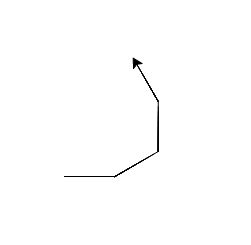
\includegraphics[width=\linewidth]{turtleExample.png}
                \caption{Interpretacja dla słowa $\alpha\beta\alpha\beta\beta\alpha\beta\alpha$, gdzie $\alpha$ to idź naprzód, a $\beta$ skręć w lewo o 30\degree.}
                \label{fig:turtleExample}
            \end{figure}
            
            Aby żółw był wstanie rysować rośliny potrzebujemy symbol pozwalający się rozgałęziać. Można osiągnąć to poprzez dodanie stosu pamiętającego aktualny stan żółwia oraz symbole na nim operujące:
            \begin{description}
                \item[{[}] - odłóż aktualny stan na stos
                \item[{]}] - ściągnij i zaaplikuj stan z góry stosu 
            \end{description}
            Stanem żółwia jest wszystko co zmienia się przy pomocy symboli np. pozycja, orientacja lub długość rysowanej linii. Rysunek \ref{fig:lsystemPlants} pokazuje przykładowe L-systemy z książki \cite{plants} 
            \begin{figure}
                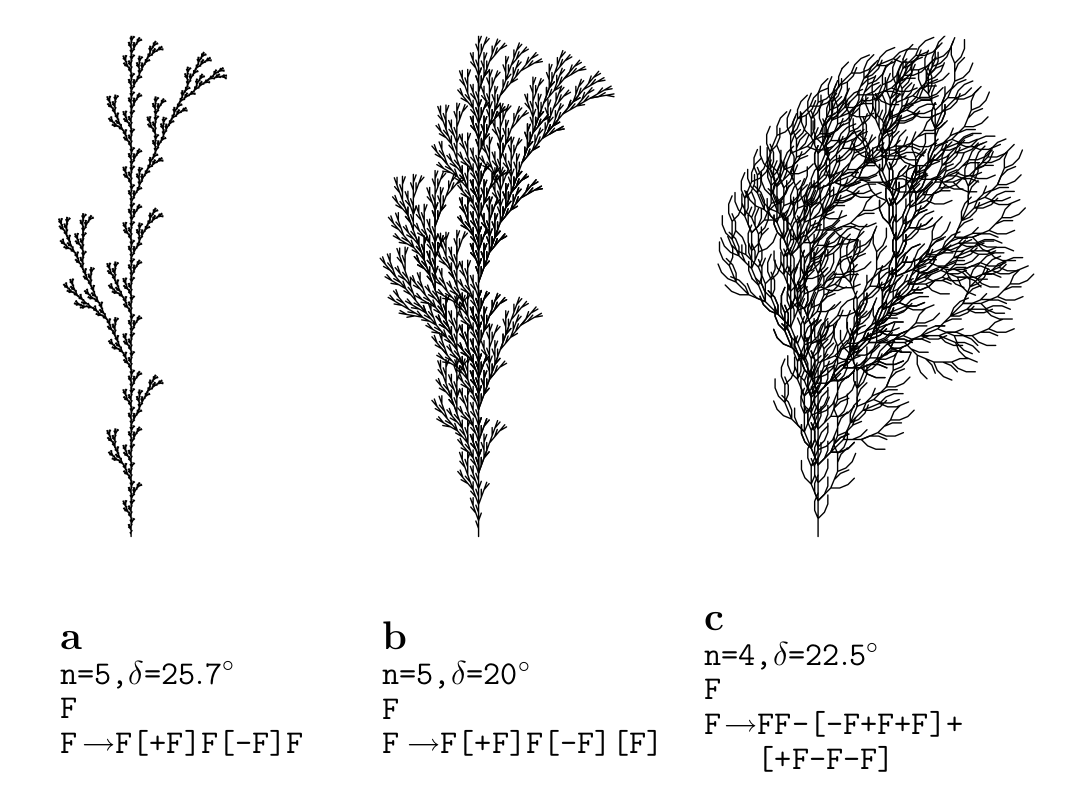
\includegraphics[width=\linewidth]{lsystemPlants.png}
                \caption{Przykład użycia symboli operujących na stosie\cite{plants}} 
                \label{fig:lsystemPlants}
            \end{figure}
            
        \subsection{Teren}
        \subsection{Tekstury}
        \subsection{Rozmieszczanie roślin}
        \subsection{Umiejscawianie kamery}
    \section{Realistyczny rendering}
        \subsection{Pathtracer}
        \subsection{Niebo}
        \subsection{Słońce}
        
\chapter{Poradnik użytkowania}

\chapter{Szczegóły programistyczne}

\chapter{Przykłady użycia}

%%%%% BIBLIOGRAFIA

\bibliographystyle{unsrt}
\bibliography{bibliography}

%\begin{thebibliography}{1}
%\bibitem{example} \ldots
%\end{thebibliography}

\end{document}
